In this section, we present the algorithm that constitutes the core of the
proposed framework for probabilistic analysis of electronic systems. The
algorithm is based on the work in \cite{jakeman2012, klimke2006, ma2009}, and it
features a sparse-grid structure, hierarchical construction, and hybrid
adaptivity. The benefits of these features are interconnected and can be
summarized as follows: the ability to efficiently tackle multidimensional
problems, the ability to perform gradual refinement of the approximation with a
natural error control, and the ability to make the refinement fine-grained and,
therefore, gain further efficiency.

Let $\f$ be a function that we would like to approximate. The function is
assumed to be in $\continuous([0, 1]^\nin)$, the space of continuous functions
in the unit hypercube $[0, 1]^\nin$. The assumption is a formality and does not
impose any restrictions in practice. In what follows, we shall gradually
construct an efficient interpolant for $\f$. Efficiency refers to the number of
function evaluations required to achieve a certain accuracy level.

\subsection{Tensor Product} \slab{tensor}
In one dimension ($\nin = 1$), $\f$ is approximated by virtue of the following
interpolation formula:
\begin{equation} \elab{tensor-1d}
  \tensor{i}(\f) = \sum_{j \in \oindex_i} \f(\x_{ij}) \, \e_{ij}
\end{equation}
where $i \geq 0$ signifies the level of interpolation; $\X_i = \{ \x_{ij} \}_{j
\in \oindex_i} \subset [0, 1]$ are the collocation nodes; $\E_i = \{ \e_{ij}
\}_{j \in \oindex_i} \subset \continuous([0, 1])$ are the basis functions; and
$\oindex_i = \{ j - 1 \}_{j = 1}^{n_i}$ is an index set enumerating (starting
from zero) the nodes and functions of level $i$. The subscript $j \in \oindex_i$
is referred to as the order of a node or function. The choice of $\X_i$ and
$\E_i$ is important and will be discussed thoroughly later on.

In multiple dimensions ($\nin > 1$), $\f$ is approximated by the tensor product
of $\nin$ one-dimensional interpolants:
\begin{equation} \elab{tensor-nd}
  \tensor{\vi}(\f) = \left( \bigotimes_{k = 1}^\nin \tensor{i_k} \right)(\f) = \sum_{\vj \in \oindex_\vi} \f(\vx_{\vi\vj}) \, \e_{\vi\vj}
\end{equation}
where $\vi = (i_k)_{k = 1}^\nin$ and $\vj = (j_k)_{k = 1}^\nin$ are
(multi-)indices specifying levels and orders, respectively, for each of the
dimensions, and $\oindex_\vi = \oindex_{i_1} \times \cdots \times
\oindex_{i_\nin}$ is an index set obtained by computing the Cartesian product of
one-dimensional index sets. In the above formula,
\begin{align}
  \X_\vi &= \X_{i_1} \times \cdots \times \X_{i_\nin} \elab{collocation-nodes} \\
         &= \left\{ \vx_{\vi\vj} = (\x_{i_k j_k})_{k = 1}^\nin \right\}_{\vj \in \oindex_\vi} \subset [0, 1]^\nin \nonumber
\end{align}
and
\begin{equation} \elab{basis-functions}
  \E_\vi = \bigotimes_{k = 1}^\nin \E_{i_k}
         = \left\{ \e_{\vi\vj} = \bigotimes_{k = 1}^\nin \e_{i_k j_k} \right\}_{\vj \in \oindex_\vi} \subset \continuous([0, 1]^\nin)
\end{equation}
are the collocation nodes and basis functions, respectively, corresponding to
index $\vi$. In \eref{basis-functions}, for any $\vx \in [0, 1]^\nin$,
\begin{equation} \elab{basis-function}
  \e_{\vi\vj}(\vx) = \left( \bigotimes_{k = 1}^\nin \e_{i_k j_k} \right)(\vx) = \prod_{k = 1}^\nin \e_{i_k j_k}(\x_k).
\end{equation}
Finally, the cardinality of $\oindex_\vi$ is as follows:
\begin{equation} \elab{tensor-cardinality}
  \n_\vi = \card{\oindex_\vi} = \prod_{k = 1}^\nin \card{\oindex_{i_k}} = \prod_{k = 1}^\nin \n_{i_k}.
\end{equation}
Equation \eref{tensor-cardinality} elucidates the prohibited expense of the
tensor-product construction shown in \eref{tensor-nd} for multidimensional
problems: the number of nodes grows exponentially as $\nin$ increases. However,
\eref{tensor-nd} serves well as a building block for more efficient algorithms,
which we discuss next.


\subsection{Smolyak Algorithm} \slab{smolyak}
One of the central algorithms in the field of multidimensional integration and
interpolation is the Smolyak algorithm \cite{smolyak1963}. Intuitively speaking,
the algorithm takes a number of small tensor-product structures and composes
them in such a way that the resulting grid has a drastically reduced number of
nodes while preserving the approximating power of the full tensor-product
construction for the classes of functions that one is typically interested in
integrating or interpolating \cite{klimke2006}.

The Smolyak interpolant for $\f$ is as follows:
\begin{equation} \elab{smolyak-original}
  \smolyak{\l}(\f) = \sum_{\l - \nin + 1 \leq |\vi| \leq \l} (-1)^{\l - |\vi|} \, {\nin - 1 \choose \l - |\vi|} \, \tensor{\vi}(\f)
\end{equation}
\updated{where $\l \geq 0$ is the index of the interpolation step, which we
shall refer to as the Smolyak level, and $|\vi| = i_1 + \dots + i_\nin$.} It can
be seen that the algorithm is indeed just a peculiar composition of
cherry-picked tensor products. However, the formula has an implication of
paramount importance. \updated{The function $\f$ needs to be evaluated only at
the nodes of the sparse grid underpinning \eref{smolyak-original}:}
\begin{equation} \elab{smolyak-grid}
  \Y_l = \bigcup_{\l - \nin + 1 \leq |\vi| \leq \l} \X_\vi.
\end{equation}
The cardinality of the above set does not have a general closed-form formula;
however, it can be several orders of magnitude smaller than the one of the full
tensor product given in \eref{tensor-cardinality}, which depends on the
dimensionality of the problem at hand and the one-dimensional rules utilized
(\sref{tensor}).

\updated{A better intuition about the properties of the Smolyak construction can
be obtained by rewriting \eref{smolyak-original} in an incremental form.} To
this end, let $\Delta\tensor{-1}(\f) = 0$,
\begin{align}
  & \Delta\tensor{i}(\f) = (\tensor{i} - \tensor{i - 1})(\f), \text{ and} \elab{tensor-delta-1d} \\
  & \Delta\tensor{\vi}(\f) = \left( \bigotimes_{k = 1}^\nin \Delta\tensor{i_k} \right)(\f). \nonumber
\end{align}
Then, \eref{smolyak-original} is identical to
\begin{equation} \elab{smolyak-incremental}
  \smolyak{\l}(\f) = \sum_{\vi \in \lindex_\l} \Delta\tensor{\vi}(\f) = \smolyak{\l - 1}(\f) + \sum_{\vi \in \Delta\lindex_\l} \Delta\tensor{\vi}(\f)
\end{equation}
where $\smolyak{-1}(\f) = 0$, and we let $\lindex_\l = \{ \vi: |\vi| \leq \l
\}$ and $\Delta\lindex_\l = \{ \vi: |\vi| = \l \}$. It can be seen that a
Smolyak interpolant can be efficiently refined: the work done in order to attain
one Smolyak level $\l$ is entirely recycled to go to the next.

\updated{The sparsity and incremental refinement of the Smolyak approach, which
are shown in \eref{smolyak-grid} and \eref{smolyak-incremental}, respectively,
are remarkable properties \perse, but they can be taken even further.} To this
end, let $\Delta\X_{-1} = \emptyset$,
\[
  \Delta\X_i = \X_i \setminus \X_{i - 1}, \text{ and } \Delta\X_\vi = \Delta\X_{i_1} \times \cdots \times \Delta\X_{i_\nin}.
\]
Then, \eref{smolyak-grid} can be rewritten as
\begin{equation} \elab{smolyak-grid-incremental}
  \Y_\l = \bigcup_{\vi \in \lindex_\l} \Delta\X_\vi = \Y_{\l - 1} \cup \bigcup_{\vi \in \Delta\lindex_\l} \Delta\X_\vi,
\end{equation}
which is analogous to \eref{smolyak-incremental}. It can be seen now that it is
beneficial to the refinement to have $\X_{i - 1}$ be entirely included in $\X_i$
since, in that case, the cardinality of $\Y_l \setminus \Y_{\l - 1} =
\bigcup_{\vi \in \Delta\lindex_\l} \Delta\X_\vi$ derived from
\eref{smolyak-grid-incremental} decreases. In words, the values of $\f$ obtained
on lower levels (lower $\l$) can be reused to attain higher levels (higher $\l$)
if the grid grows without abandoning its previous structure. With this in mind,
the rule used for generating successive sets of points $\{ \X_i \}_i$ should be
chosen to be nested, that is, in such a way that $\X_i$ contains all nodes of
$\X_{i - 1}$.

The final step in this subsection is to rewrite \eref{smolyak-incremental} in a
hierarchical form. To this end, we require the interpolants of higher levels to
represent exactly the interpolants of lower levels. In one dimension, it means
that
\begin{equation} \elab{tensor-exactness}
  \tensor{i - 1}(\f) = \tensor{i}(\tensor{i - 1}(\f)).
\end{equation}
The condition in \eref{tensor-exactness} can be satisfied by an appropriate
choice of collocation nodes and basis functions, which will be discussed later.
If \eref{tensor-exactness} holds, using \eref{tensor-1d} and
\eref{tensor-delta-1d},
\[
  \Delta\tensor{i}(\f) = \sum_{j \in \Delta\oindex_i} \left( \f(\x_{ij}) - \tensor{i - 1}(\f)(\x_{ij}) \right) \, \e_{ij}
\]
where $\Delta\oindex_i = \{ j \in \oindex_i: \x_{ij} \in \Delta\X_i \}$. The
above sum is over $\Delta\X_i$ due to the fact that the difference in the
parentheses is zero whenever $\x_{ij} \in \X_{i - 1}$ since $\X_{i - 1} \subset
\X_i$.

In multiple dimensions, using the Smolyak formula,
\begin{equation} \elab{tensor-delta}
  \Delta\tensor{\vi}(\f) = \sum_{\vj \in \Delta\oindex_\vi} \left( \f(\vx_{\vi\vj}) - \smolyak{|\vi| - 1}(\f)(\vx_{\vi\vj}) \right) \, \e_{\vi\vj}
\end{equation}
where $\Delta\oindex_\vi = \{ \vj \in \oindex_\vi: \vx_{\vi\vj} \in
\Delta\X_\vi \}$. The delta
\begin{equation} \elab{surplus}
  \surplus(\vx_{\vi\vj}) = \f(\vx_{\vi\vj}) - \smolyak{|\vi| - 1}(\f)(\vx_{\vi\vj})
\end{equation}
is called a hierarchical surplus. When increasing the interpolation level, this
surplus is nothing but the difference between the actual value of $\f$ at a new
node and the approximation of this value computed by the interpolant constructed
so far.

The final formula for nonadaptive hierarchical interpolation is obtained by
substituting \eref{tensor-delta} into \eref{smolyak-incremental}:
\begin{align}
  \smolyak{\l}(\f) &= \sum_{\vi \in \lindex_\l} \, \sum_{\vj \in \Delta\oindex_\vi} \surplus(\vx_{\vi\vj}) \, \e_{\vi\vj} \nonumber \\
                   &= \smolyak{\l-1}(\f) + \sum_{\vi \in \Delta\lindex_\l} \, \sum_{\vj \in \Delta\oindex_\vi} \surplus(\vx_{\vi\vj}) \, \e_{\vi\vj} \elab{smolyak-hierarchical}
\end{align}
where $\surplus(\vx_{\vi\vj})$ is computed according to \eref{surplus}.


\begin{figure}[t]
  \centering
  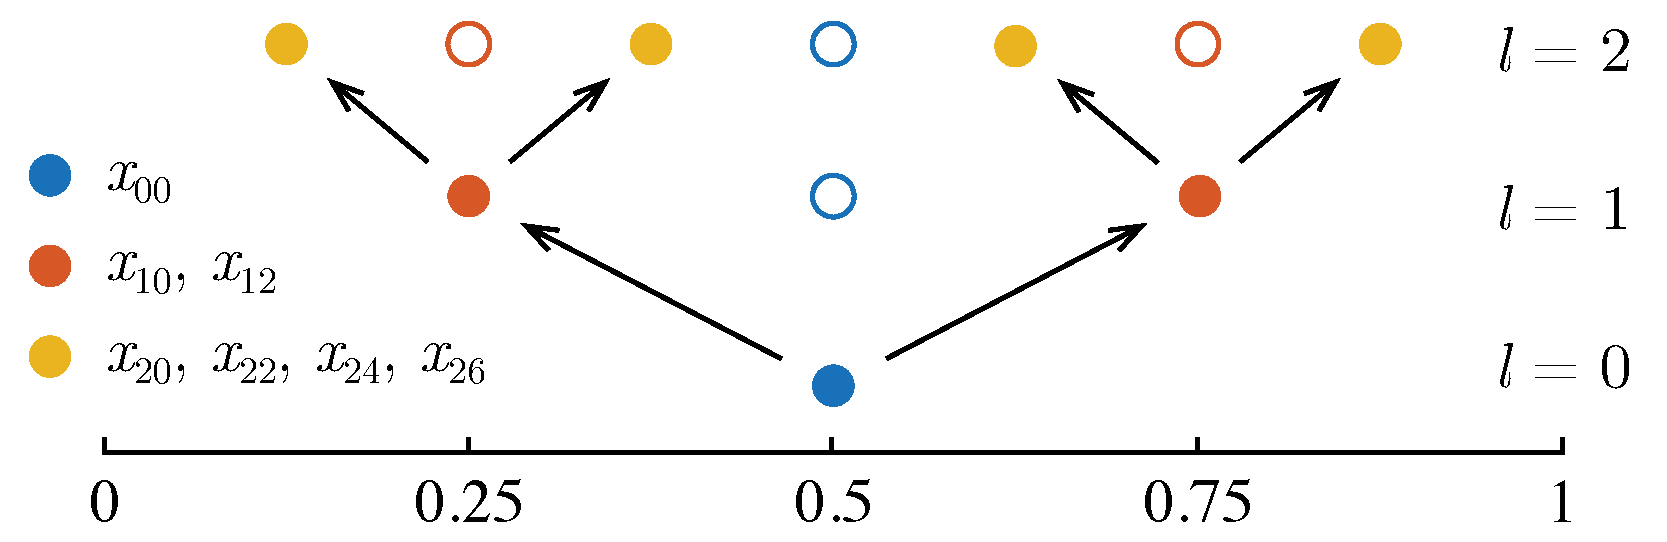
\includegraphics[width=1.0\columnwidth]{include/assets/figures/grid.pdf}
  \vspace{-1.5em}
  \caption{
    The open Newton--Cotes rule for the first three level of one-dimensional
    hierarchical interpolation.
  }
  \flab{grid}
\end{figure}

\subsection{Collocation Nodes} \slab{grid}
A sparse grid that is fully nested and, moreover, well disposed to adaptivity,
as we shall see, can be constructed using the (one-dimensional) Newton--Cotes
rule \cite{ma2009}. For each level, the rule is merely a set of equidistant
nodes on $[0, 1]$.

The rule comes in two flavors: closed and open. The only difference between the
two is that the former includes the endpoints, that is, 0 and 1, while the
latter does not. Now, in \sref{smolyak}, we postulated that the assumption in
\eref{tensor-exactness} was needed in order to proceed. The closed rule
satisfies this assumption, and it is the one used in the original version of
local adaptivity presented in \cite{ma2009}. The open Newton--Cotes rule, on the
other hand, violates the assumption close to the boundaries of the interval.
However, we found that the open rule is a viable option since it performs well
in practice, which was also noted in \cite{klimke2006}. In fact, we were able to
obtain better results with the open rule and decided to present it here.

The open Newton--Cotes rule of level $i \geq 0$ is
\begin{equation} \elab{newton-cotes-grid}
  \X_i = \left\{ x_{ij} = \frac{j + 1}{\n_i + 1} \right\}_{j \in \oindex_i}
\end{equation}
where $\oindex_i = \left\{ i - 1 \right\}_{i = 1}^{\n_i}$ and $\n_i = 2^{i + 1}
- 1$. The first three levels of the rule are depicted in \fref{grid}. It can be
seen that the number of nodes (in one dimension) grows as 1, 3, 7, 15, 31, and
so on, and that the rule is fully nested. In multiple dimensions, the nodes are
formed as shown in \eref{collocation-nodes}.


\begin{figure}[t]
  \centering
  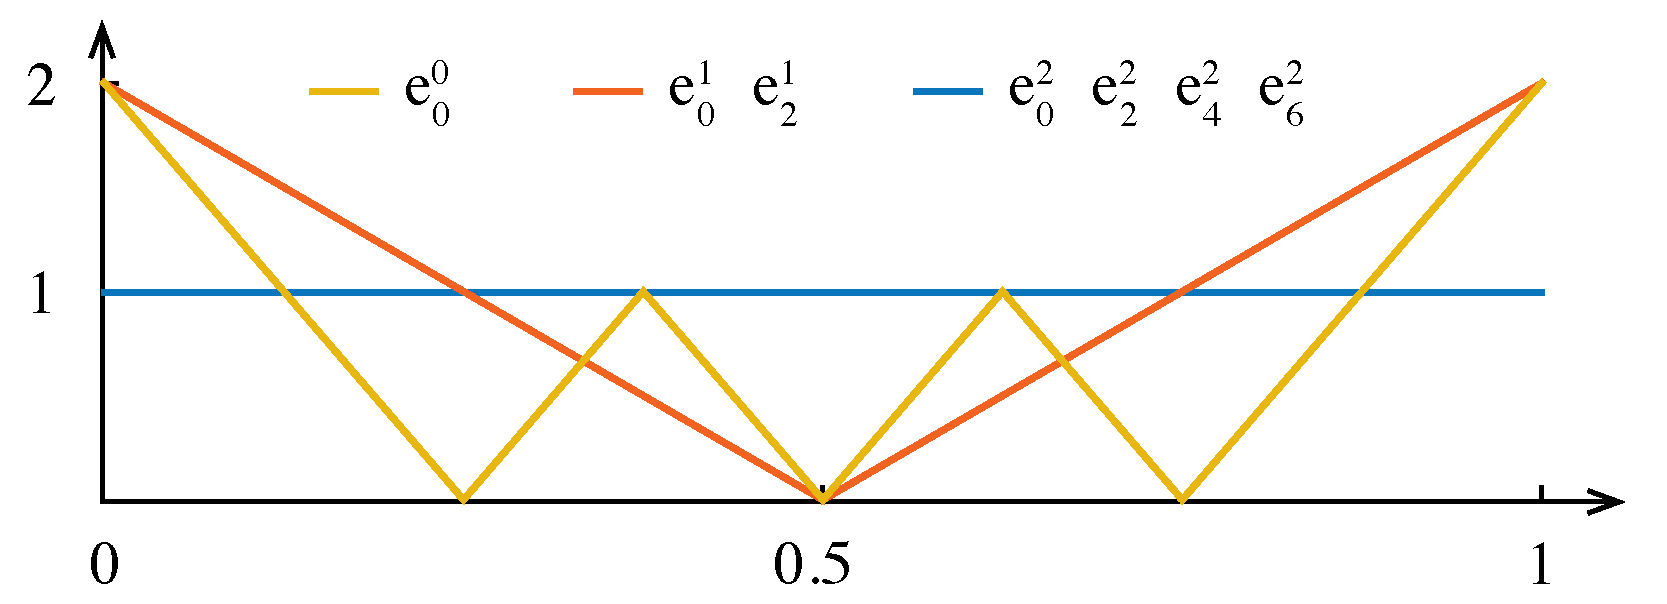
\includegraphics[width=1.0\columnwidth]{include/assets/figures/basis.pdf}
  \vspace{-1.5em}
  \caption{
    The first three levels of the basis described in \sref{basis}.
  }
  \flab{basis}
\end{figure}

\subsection{Basis Functions} \slab{basis}
\updated{The basis functions that correspond the open Newton--Cotes rule
described in \sref{grid} are the following piecewise linear functions.} For $i =
0$ and $j = 0$, we have that $\e_{00}(\x) = 1$. For $i > 0$ and $j = 0$ (close
to the left endpoint),
\[
  \e_{i0}(\x) = \begin{cases}
    2 - \left( \n_i + 1 \right) \x, & \text{if } \x < \frac{2}{\n_i + 1}, \\
    0, & \text{otherwise}.
  \end{cases}
\]
For $i > 0$ and $j = \n_i - 1$ (close to the right endpoint),
\[
  \e_{i(\n_i - 1)}(\x) = \begin{cases}
    \left( \n_i + 1 \right) \x - \n_i + 1, & \text{if } \x > \frac{\n_i - 1}{\n_i + 1}, \\
    0, & \text{otherwise}.
  \end{cases}
\]
In other cases,
\[
  \e_{ij}(\x) = \begin{cases}
    1 - \left( \n_i + 1 \right)|\x - \x_{ij}|, & \text{if } |\x - \x_{ij}| < \frac{1}{\n_i + 1}, \\
    0, & \text{otherwise}.
  \end{cases}
\]
The basis functions corresponding to the first three levels of one-dimensional
interpolation are depicted in \fref{basis}. In multiple dimensions, the basis
functions are formed as shown in \eref{basis-functions}.

Lastly, let us mention the volumes (integrals over the whole domain) of the
basis functions denoted by $\w_{ij}$; they will be needed in continuation.
Namely, $\w_{00} = 1$ and, for $i > 0$,
\begin{equation} \elab{volume}
  \w_{ij} = \int_0^1 \e_{ij}(\x) \, \d\x = \begin{cases}
    \frac{2}{\n_i + 1}, & \text{if } j \in \{ 0, \n_i - 1 \}, \\
    \frac{1}{\n_i + 1}, & \text{otherwise}.
  \end{cases}
\end{equation}
In multiple dimensions, the volumes are products of the one-dimensional
components, analogous to \eref{basis-function}.

Imagine now a function that is nearly flat on the first half of $[0, 1]$ and
rather irregular on the other. Under these circumstances, it is natural to
expect that, in order to attain the same accuracy, the first half would require
much fewer collocation nodes than the other one; recall \fref{motivation}.
However, if we followed the construction procedure described so far, we would
not be able to benefit from this peculiar behavior: we would treat both sides
equally and would add all the nodes of each level. The solution to the above
problem is to make the interpolation algorithm adaptive, which we shall discuss
next.


\subsection{Adaptivity} \slab{adaptivity}
Imagine a function that is nearly flat on the first half of $[0, 1]$ and rather
irregular on the other. Under these circumstances, it is natural to expect that,
in order to attain the same accuracy, the first half would require much fewer
collocation nodes than the other one; recall \fref{motivation}. However, if we
followed the construction procedure described so far, we would not be able to
benefit from the peculiar behavior: we would treat both sides equally and would
add all the nodes of each level.

The solution to the above problem is to make the interpolation algorithm
adaptive. To this end, we first need to find a way to measure how good our
approximation is at any point in the domain of $\f$. Then, when refining the
interpolant, instead of bombarding $\f$ with all possible nodes, we will only
choose those that are located in the regions with poor accuracy as indicated by
the yet-to-be-found accuracy metric.

Thanks to the hierarchical form obtained in the previous subsection, we already
have a good material for building an accuracy metric. Recall \eref{surplus}.
Hierarchical surpluses are natural indicators of the interpolation error: they
are the difference between the true function and its approximation at the nodes
of the underlying sparse grid. Hence, they can be recycled in order to
effectively identify ``problematic'' regions. Specifically, we first assign a
score to each node $\vx_{\vi\vj}$ or, equivalently, to each pair of level and
order indices $(\vi, \vj)$:
\begin{equation} \elab{score}
  \score_{\vi\vj} = \left| \surplus(\vx_{\vi\vj}) \, \w_{\vi\vj} \right|
\end{equation}
where $\surplus(\vx_{\vi\vj})$ and $\w_{\vi\vj}$ are given by \eref{surplus} and
\eref{volume}, respectively, and this score is then used in order to guide the
algorithm as we shall explain in the rest of this subsection.

The Smolyak construction in \eref{smolyak-hierarchical} is rewritten as follows:
\begin{equation} \elab{approximation}
  \approximation{\l}(\f) = \approximation{\l-1}(\f) + \sum_{\vi \in \Delta\lindex_\l} \sum_{\vj \in \Delta\oindex_\vi} \surplus(\vx_{\vi\vj}) \,
\e_{\vi\vj}.
\end{equation}
The main different with respect to \eref{smolyak-hierarchical} is that $\l \geq
0$ no longer signifies a Smolyak level but a more abstract interpolation step,
and $\approximation{\l}$ is the interpolant at that step. As always,
$\approximation{-1} = 0$, and the definition of $\surplus$ given in
\eref{surplus} is adjusted accordingly. Lastly, all index sets from now on are
generally subsets of their full-fledged counterparts defined in
\sref{smolyak-algorithm}.

\begin{remark}
All the rules below make sure that the construction in \eref{approximation}
adhere to the same principles as the ones underpinning
\eref{smolyak-hierarchical}. An arbitrary construction is generally invalid.
\end{remark}

Each $\approximation{\l}$ is characterized by a set of level indices
$\lindex_\l$, and each $\vi \in \lindex_\l$ by a set of order indices
$\Delta\oindex_\vi$. At each interpolation step $\l \geq 0$, a single index
$\vi_\l$ is chosen from $\lindex_{\l-1}$ with $\lindex_{-1} = \{ \v{0} \}$. The
chosen index then gives birth to $\Delta\lindex_\l$ and $\{ \Delta\oindex_\vi
\}_{\vi \in \Delta\lindex_\l}$, which shape the increment in the right-hand side
of \eref{approximation}.

The set $\Delta\lindex_\l$ contains the so-called admissible forward neighbors
of $\vi_\l$. Let us now parse the previous sentence. First, the forward
neighbors of an index $\vi$ are given by
\begin{equation} \elab{forward-level-neighbors}
  \left\{ \vi + \v{1}_k: k = 1, \dots, \nin \right\}
\end{equation}
where $\v{1}_k$ is a vector whose elements are zero except for element $k$ equal
to unity. Next, an index $\vi$ is admissible if its inclusion into the index set
in question $\lindex$ keeps the set admissible. Finally, $\lindex$ is admissible
if it satisfies the following condition \cite{klimke2006}:
\begin{equation} \elab{admissibility}
  \vi - \v{1}_k \in \lindex, \text{ for $\vi \in \lindex$ and $k = 1, \dots, \nin$,}
\end{equation}
where, naturally, the cases with $i_k = 0$ need no check.

Now, how is $\vi_\l$ chosen from $\lindex_{\l-1}$ at each iteration of
\eref{approximation}? First of all, each index can be obviously picked at most
once. The rest is resolved by prioritizing the candidates. It is reasonable to
assign a priority to a level index $\vi$ based on the scores of the order
indices associated with it, that is, on the scores of $\oindex_\vi$. We compute
the priority as the average score:
\[
  \score_\vi = \frac{1}{\card{\Delta\oindex_\vi}} \sum_{\vj \in \Delta\oindex_\vi} \score_{\vi\vj}
\]
Consequently, the answer to the above question is that, at each step $\l$, the
index $\vi$ with the highest $\score_\vi$ gets promoted to $\vi_\l$.

Let us now turn to the content of $\Delta\oindex_\vi$ where $\vi = \vi_\l +
\v{1}_k$ for a fixed $k$. It also contains admissible forward neighbors, but
they are order indices, and their construction is drastically different from the
one in \eref{forward-level-neighbors}. Concretely, these indices are identified
by inspecting the backward neighborhood of $\vi$ (analogous to
\eref{forward-level-neighbors}). For each backward neighbor $\hat{\vi} = \vi -
\v{1}_{\hat{k}}$ and each $\vj \in \Delta\oindex_{\hat{\vi}}$, we begin by
checking the following condition:
\[
  \score_{\hat{\vi}\vj} \geq \serror
\]
where $\serror$ is a user-defined constant referred to as the score error. If
the condition holds, the forward neighbors of $\vj$ in dimension $k$ are added
to $\Delta\oindex_\vi$. This procedure for the open Newton--Cotes rule is
illustrated in \fref{rule}. The arrows emerging from a node connect the node
with its forward neighbors. It can be seen that each node has two forward
neighbors (for one dimension); their order indices are
\[
  (j_1, \dots, 2 j_k, \dots, j_\nin) \hspace{1em} \text{and} \hspace{1em} (j_1, \dots, 2 j_k + 2, \dots, j_\nin).
\]
The above refinement procedure is repeated for each index $\vi \in
\Delta\lindex_\l$ with respect to each dimension $k = 1, \dots, \nin$.

The final question is the stopping condition of the approximation process in
\eref{approximation}. Apart from the obvious constraints on the maximum number
of function evaluations and deepness of interpolation (the Smolyak level), we
rely on the following criterion. Assume given two additional constants:
$\aerror$ and $\rerror$ referred to as the absolute and relative error,
respective. Then, the process is terminated as soon as
\[
  \max_{(\vi, \vj)} \, |\surplus(\vx_{\vi\vj})| \leq \max \left\{ \aerror, \, \rerror (\f_\text{max} - \f_\text{min}) \right\}
\]
where $\f_\text{min}$ and $\f_\text{max}$ the minimum and maximum observed
values of $\f$, respectively, and the left-hand side is the maximum surplus
whose level index has not been refined yet (considered as $\vi_\l$ at some step
$\l$ in \eref{approximation}). The above criterion is a sound way to curtail the
process it is based on the actual progress.

The adaptivity presented in this subsection is referred to as hybrid as it
exhibits features of both global and local adaptivity. Local adaptivity operates
on the level of individual nodes, and it has already been motivated. Global
adaptivity operates on the level of individual dimensions. The intuition behind
it is that, in general, the input variables manifest themselves (impact $\f$)
differently, and the interpolation algorithm is likely to benefit by
prioritizing those variables that the most influential.


To summarize, we have obtained an efficient algorithm for adaptive hierarchical
interpolation in multiple dimensions. The main equation is \eref{approximation}
where $\surplus$, $\vx_{\vi\vj}$, and $\e_{\vi\vj}$ are the ones given in
\sref{smolyak}, \sref{grid}, and \sref{basis}, respectively, and the
interpolation procedure is undertaken according to the rules given in
\sref{adaptivity}. In the next subsection, we shall discuss the algorithmic
structure of our interpolation.

\subsection{Implementation} \slab{implementation}
The life cycle of interpolation has roughly two stages: construction and usage.
The construction stage invokes $\f$ at a set of collocation nodes and produces
certain artifacts. The usage stage estimates the values of $\f$ at a set of
arbitrary points by manipulating the artifacts. In this subsection, we shall
look at the pseudocodes of the two stages. The purpose is to give the big
picture. A lot of implementation details are purposely omitted; however, all the
details can be found and studied online as our implementation is open source
\cite{sources}.

Let us first make a general note. We found it beneficial to the clarity and ease
of implementation to collapse the two sums in \eref{approximation} into one.
This requires storing a level index $\vi = (i_k)_{k = 1}^\nin$ and an order
index $\vj = (j_k)_{k = 1}^\nin$ for each interpolation element. It is also
advantageous to encode each pair $(i_k, j_k)$ as a single unsigned integer,
which, in particular, eliminates excessive memory usage. In multiple dimensions,
this results in a single vector $\vl = (\iota_k)_{k = 1}^\nin$, which we simply
call an index. The encoding that we utilize is as follows:
\[
  \iota_k = i_k \lor (j_k \ll \n_\text{bits})
\]
where $\lor$ and $\ll$ are the bitwise \up{OR} and logical left shift,
respectively, and $\n_\text{bits}$ is the number of bits reserved for storing
Smolyak levels, which can be adjusted according to the maximum permitted
deepness of interpolation.

The pseudocode of the construction stage is given in \aref{construct} called
\token{Construct}. The \token{target} input is a function $\f$ to be
approximated. The \token{surrogate} output is a structure containing the
artifacts of interpolation, which are a set of tuples $\{ (\vl_k,
\surplus(\vx_{\vl_k}) \}_k$, giving a comprehensive description of an
interpolant. The routine works as follows.

\begin{compactlist}

\point{Line~2:} Each iteration is an interpolation step in \eref{approximation}.
It has a state captured by a structure denoted by \token{s}. The
\token{strategy} object represents an adaptation strategy utilized and works as
described in \sref{adaptivity}. The \token{First} method of \token{strategy}
returns the initial state of the first step so that the \token{indices} field of
\token{s} is initialized with the indices of that step. The body of the loop
populates the rest of the fields of \token{s} so that \token{strategy.Next} can
adequately produce the initial state of the next iteration. The process
terminates when a stopping condition is satisfied, in which case \token{Next}
returns a null state.

\point{Line~3:} The \token{grid} object represents the interpolation grid
utilized (see \sref{grid}), and its \token{Compute} method converts the step's
indices into the coordinates of the corresponding collocation nodes, that is,
$\{ \vl_k \}_k$ into $\{ \vx_{\vl_k} \}_k$.

\point{Line~4:} \token{Invoke} evaluates \token{target} at the collocation
nodes. This is a prominent candidate for parallelization since the algorithm
does not impose any evaluation order; $\f$ can be calculated simultaneously for
all the nodes of the iteration.

\point{Line~5:} \token{Evaluate} exercises the interpolant constructed so far at
the collocation nodes, approximating the values obtained on line~4. This
function will be discussed separately.

\point{Line~6:} \token{Subtract} computes the difference between the true and
approximated values of \token{target}, which yields the step's hierarchical
surpluses $\{ \surplus(\vx_{\vl_k}) \}_k$, similar to \eref{surplus}.

\point{Line~7:} \token{strategy.Score} calculates the scores of the new
collocation nodes based on their surpluses; see \eref{score}.

\point{Line~8:} \token{Append} improves the interpolant by extending it with the
indices and surpluses of the current iteration.

\end{compactlist}

We now turn to the usage stage of an interpolant. The pseudocode is given in
\aref{evaluate} called \token{Evaluate}. This algorithm is also involved in
\aref{construct}; see line~5. Let us make a couple of observations regarding
\token{Evaluate}.

\begin{compactlist}

\point{Line~4:} The inner loop is an unfolded version of \eref{approximation}
(there is no separation between individual interpolation steps taken).

\point{Line~5:} The \token{basis} object represents the interpolation basis
utilized (see \sref{basis}), and its \token{Compute} method evaluates a single
(multidimensional) basis function at a single point.

\end{compactlist}

It is worth noting that the \token{basis}, \token{grid}, and \token{strategy}
objects conform to certain interfaces and can be easily swapped out. This makes
the two algorithms very general and reusable with different configurations. In
particular, the adaptation strategy can be fine-tuned for each particular
problem.


To recapitulate, in this section, we have presented the key component of the
proposed framework for probabilistic analysis of electronic systems: an
efficient approach to multidimensional interpolation. The interpolation
technique is based on the Smolyak algorithm, which enables the interpolation to
be performed in an adaptive hierarchical manner, highly beneficial for practical
computations. The overall technique has been consolidated in \aref{construct}
and \aref{evaluate}.
